%%%%%%%%%%%%%%%%%%%%%%%%%%%%%%%%%%%%%%%%%%%%%%%%%%%%%%%%%%%%%%%%%%%%%%%%%%%%%%
%% Beamer style for JDOC A1 poster
%%%%%%%%%%%%%%%%%%%%%%%%%%%%%%%%%%%%%%%%%%%%%%%%%%%%%%%%%%%%%%%%%%%%%%%%%%%%%%

%-- A1 beamer slide ----------------------------------------------------------
\documentclass[final, xcolor={usenames, dvipsnames}]{beamer}
\usepackage[
  orientation=portrait,
  scale=1.25,           % font scale factor
  size=a1               % poster format
]{beamerposter}

\usepackage[utf8]{inputenc}
\usetheme[facepic=include/id_picture2.eps]{JDOC}

% Additional packages
\usepackage{booktabs}
\usepackage{ragged2e}
\usepackage{overpic}

%\colorlet{colorprimary}{skyblue1}
%\colorlet{colorsecondary}{skyblue2}
%\colorlet{colortertiary}{skyblue3}
%\colorlet{colorquaternary}{colortertiary!50!black}
\colorlet{colorprimary}{CornflowerBlue}
\colorlet{colorsecondary}{colorprimary!75!black}
\colorlet{colortertiary}{colorsecondary!50!black}
\colorlet{colorquaternary}{colortertiary!25!black}
\beamertemplatesolidbackgroundcolor{white}

\addtobeamertemplate{block begin}{}{\justifying}
\addtobeamertemplate{item}{}{\justifying}
\setbeamertemplate{caption}{\insertcaption}

%-- Title and authors of the poster ------------------------------------------
\title{\Huge\textbf
  Extraction automatique de termes-clés\\à partir de sujets
}

\author{
  Adrien BOUGOUIN\\
  E-mail : adrien.bougouin@univ-nantes.fr
}

\institute{%
  Spécialité : Informatique\\ % Research category
  Laboratoire : LINA\\        % Laboratory name
  \'{E}quipe : TALN           % Team name
}

\begin{document}
  \begin{frame}[b]{}
    %-- Introduction -----------------------------------------------------------
    \begin{columns}[t]
      \begin{column}{.45\linewidth}
        \begin{block}{Problématique}
          \begin{itemize}
            \item{Les termes-clés sont des unités textuelles capables de
                  synthétiser le contenu d'un document}
            \item{Quelle est la nature linguistique des termes-clés~?}
            \item{Comment distinguer les termes-clés des autres unités
                  textuelles de même nature linguistique~?}
          \end{itemize}
        \end{block}
      \end{column}

      \begin{column}{.45\linewidth}
        \begin{block}{Solution proposée}
          \vspace{.55em}
          \begin{enumerate}
            \item{Extraction des groupes nominaux du document}
            \item{Groupement des groupes nominaux en sujets (concepts)}
            %\item{Modélisant du lien sémantique entre chaque sujet}
            \item{Ordonnancement par importance des sujets}
            \item{Sélection d'un terme-clé pour chaque sujet}
          \end{enumerate}
          \vspace{.59em}
        \end{block}
      \end{column}
    \end{columns}

    \vspace{-1em}

    %-- Example et conclusion  -------------------------------------------------
    \begin{columns}[b]
      \begin{column}{.45\linewidth}
        \section{\textcolor{white}{Exemple~:}}

        \vspace{.25em}

        \begin{columns}
          \begin{column}{.36\linewidth}
            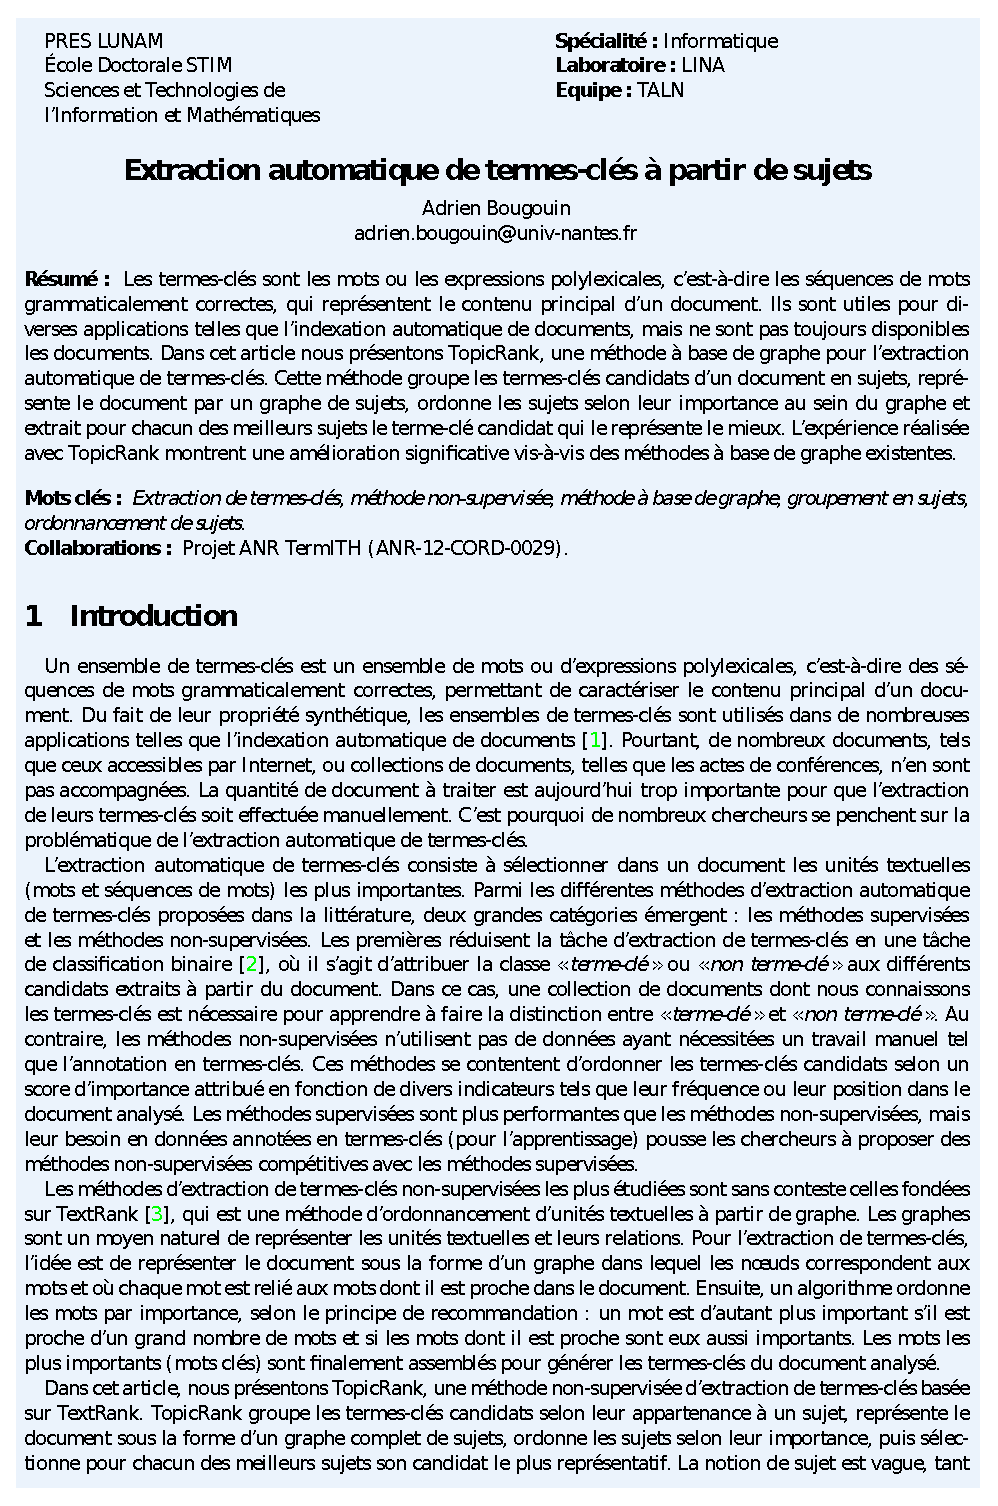
\includegraphics[width=\linewidth]{include/BOUGOUIN_LINA_papier_mod.eps}
            \vspace{12.5em}
          \end{column}\hfill

          \begin{column}{.45\linewidth}
            \small
            \begin{center}
              \begin{table}
                \caption{Sujets}
                \begin{tabular}{|@{~-~}l|}
                  \hline
                  sujets \hfill \underline{\textit{s1}}\\
                  meilleurs sujets\\
                  \hline
                  termes-clés \hfill \underline{\textit{s2}}\\
                  termes-clés candidats\\
                  \hline
                  document \hfill \underline{\textit{s3}}\\
                  \hline
                  \dots\\
                  \hline
                \end{tabular}
              \end{table}

              \vspace{.75em}

              \begin{overpic}[width=.5\linewidth,angle=180]{include/arrow.eps}
              %\begin{overpic}[grid,tics=5,width=.5\linewidth,angle=180]{include/arrow.eps}
                \put(69, 50){\small (2) Groupement lexical}
                \put(94, 30){\small des groupes nominaux}
                \put(94, 10){\small (s'ils partagent $^\text{1}\text{\small /}_\text{\footnotesize 4}$ de}
                \put(94, -10){\small leurs mots)}

                % other arrows
                \put(-141.5, -56){
                  \begin{overpic}[width=.5\linewidth,angle=55]{include/arrow.eps}
                  %\begin{overpic}[grid,tics=5,width=.5\linewidth,angle=55]{include/arrow.eps}
                    \put(-54, 37.5){\small (1) Extraction des}
                    \put(-36, 22.5){\small plus longues}
                    \put(-36, 7.5){\small séquences de noms,}
                    \put(-36, -7.5){\small noms propres et}
                    \put(-36, -22.5){\small adjectifs}
                  \end{overpic}
                }
                \put(173.5, 115){
                  \begin{overpic}[width=.5\linewidth,angle=90]{include/arrow.eps}
                  %\begin{overpic}[grid,tics=5,width=.5\linewidth,angle=90]{include/arrow.eps}
                  \end{overpic}
                }
              \end{overpic}

              \vspace{.75em}

              \begin{table}
                \begin{tabular}{|@{~-~}l|}
                  \hline
                  sujets\\
                  meilleurs sujets\\
                  termes-clés\\
                  termes-clés candidats\\
                  document\\
                  \dots\\
                  \hline
                \end{tabular}
                \caption{Groupes nominaux}
              \end{table}
            \end{center}
          \end{column}
        \end{columns}

        \begin{block}{Résultats}
          \begin{itemize}
            \item{Comparaison de TopicRank avec TextRank~\cite{mihalcea2004textrank}}
            \item{Application à 100 articles journalistiques (WikiNews)}
            \item{Extraction de 10 termes-clés par document}
          \end{itemize}
          \begin{table}
            \centering
            \begin{tabular}{r|ccc}
              \toprule
              \textbf{Méthode} & \textbf{Précision} & \textbf{Rappel} & \textbf{F-mesure}\\
              \hline
              %TF-IDF~\cite{jones1972tfidf} & 33,9 & 35,9 & 34,3\\
              TextRank & $~~$9,3 & $~~$8,3 & $~~$8,6\\
              %SingleRank~\cite{wan2008expandrank} & 19,4 & 20,7 & 19,7\\
              \textbf{TopicRank} & \textbf{35,0} & \textbf{37,5} & \textbf{35,6}\\
              \bottomrule
            \end{tabular}
          \end{table}
        \end{block}
      \end{column}

      \begin{column}[b]{.45\linewidth}
        \begin{center}
          \begin{figure}
            \caption{Modélisation du lien sémantique entre chaque sujet}
            \begin{overpic}[width=.5\linewidth]{include/graph_mod.eps}
            %\begin{overpic}[grid,tics=5,width=.5\linewidth]{include/graph_mod.eps}
              \put(78, 87.5){\scriptsize arête pondérée selon la force du lien}
              \put(83, 82.5){\scriptsize sémantique entre s1 et s19}
            \end{overpic}
          \end{figure}

          \vspace{.5em}

          \begin{overpic}[width=.25\linewidth]{include/arrow.eps}
          %\begin{overpic}[grid,tics=5,width=.25\linewidth]{include/arrow.eps}
            \put(-89, 75){\small (3) Ordonnancement}
            \put(-67, 57.5){\small des sujets, selon}
            \put(-67, 40){\small TextRank~\cite{mihalcea2004textrank}}

            \put(68, 57.5){\small (4) Pour les $k$ meilleurs sujets~:}
            \put(90, 40){\small extraction du groupe}
            \put(90, 22.5){\small nominal apparaissant en}
            \put(90, 5){\small premier dans le document}
          \end{overpic}

          \begin{figure}
            
\includegraphics[width=.875\linewidth]{include/word_cloud.eps}
            \caption{Termes-clés}
          \end{figure}
        \end{center}
        \begin{block}{Perspectives}
          \begin{itemize}
            \item{Usage de connaissances linguistiques pour le groupement en
                  sujets}
            \item{Exploration de diverses stratégies de selection du terme-clé
                  le plus représentatif d'un sujet}
          \end{itemize}
        \end{block}
      \end{column}
    \end{columns}

    \bigskip

    %-- References -------------------------------------------------------------
    \begin{columns}
      \begin{column}{.95\linewidth}
        \setbeamerfont{block title}{size=\normalsize}
        \begin{block}{Références}
          \bibliographystyle{unsrt}
          \bibliography{../../biblio}
        \end{block}
      \end{column}
    \end{columns}

    %-- Aknowledgement ---------------------------------------------------------
    \begin{columns}
      \begin{column}{.2\linewidth}
        
\includegraphics[width=\linewidth]{include/termith.eps}
        \vspace{1em}
      \end{column}

      \begin{column}{.75\linewidth}
        Ce travail a bénéficié d'une aide de l'Agence Nationale de la Recherche
        portant la référence (ANR-12-CORD-0029).
      \end{column}
    \end{columns}
    \vspace{.5cm}
  \end{frame}
\end{document}

